\documentclass{awesomecv}

\usepackage{geometry}
\geometry{
  left  =  30mm,
  right =  30mm,
  bottom = 40mm,
  top =    40mm
}

\documentcolor{blue}
\secondcolor{base01}
\thirdcolor{base01}
\sectioncolor{base02}

\titlethicknessleft{3mm}

\voiceleftsize{2.1cm}
\voicerightsize{12cm}

\begin{document}

\begin{titlebox}
  \authorname{Raoul Wols}{\emph{curriculum vit\ae}}

  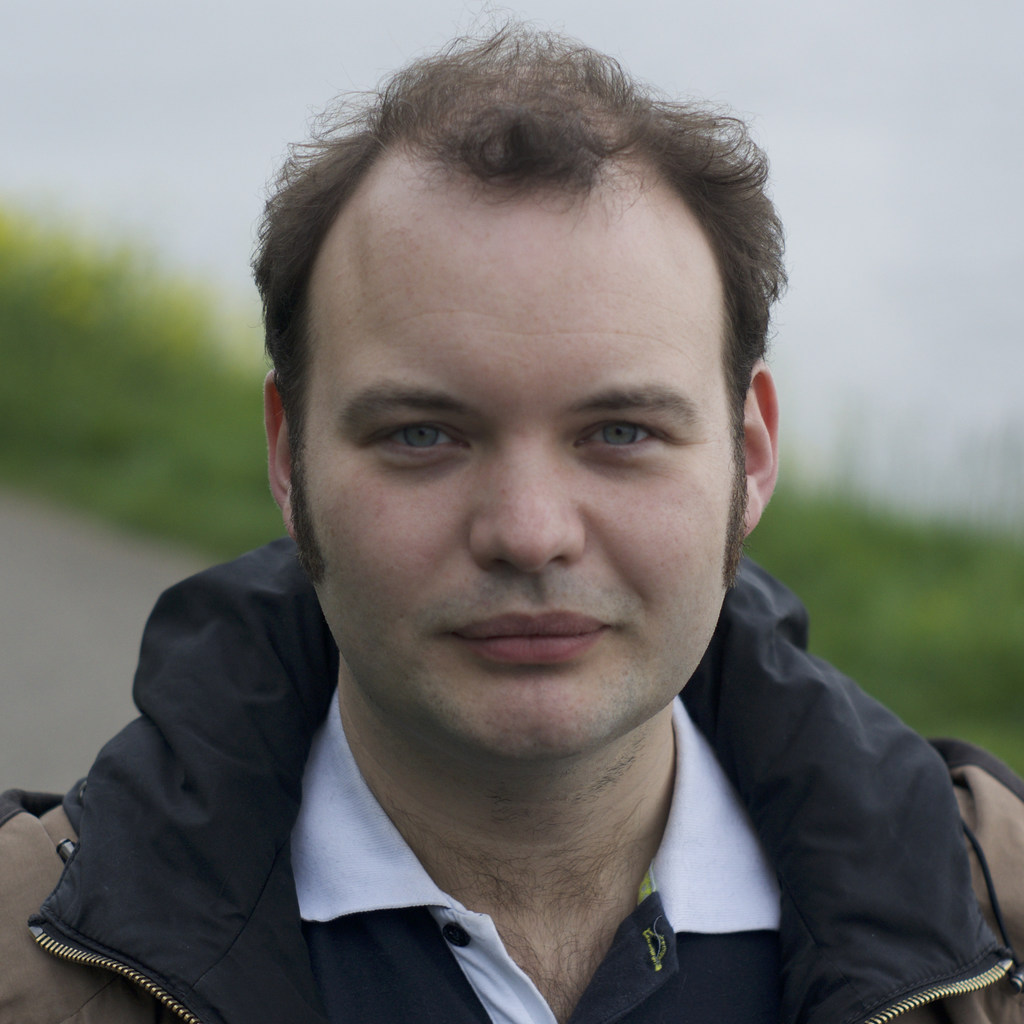
\includegraphics[scale=.2]{pics/me.jpg}
  % \qrcode{pics/qrcode.png}

  \tcblower

  \begin{showinfo}
    \birthdate{January 19th, 1989}
    \location{Slobbengorsweg 129}
    \location{3351LH Papendrecht}
    \location{The Netherlands}
    \mobile{+31 (0) 6 10917383}
    \firstMail{raoulwols@gmail.com}
    \firstMail{r@primef.actor}
    \github{https://github.com/rwols}
    \stackoverflow{stackoverflow.com/users/990142}
    \twitter{https://twitter.com/rwols}
    \website{http://primef.actor}
  \end{showinfo}

\end{titlebox}

\updated{\today}

\opensection{\faGraduationCap}{Education}
\begin{describesection}

  \leftside{from \textbf{sep 2001} to \textbf{june 2007}}
  \rightsidecomplex{Gymnasium}{Johan de Witt Gymnasium}{Dordrecht, The Netherlands}{\;}

  \leftside{from \textbf{sep 2007} to \textbf{june 2010}}
  \rightsidecomplex{Minor Jazz Piano}{Royal Conservatory of The Hague}{The Hague, The Netherlands}{Final grade: 7.5}

  \leftside{from \textbf{sep 2007} to \textbf{july 2012}}
  \rightsidecomplex{Bachelor of Science in Mathematics}{Leiden University}{Leiden, The Netherlands}{Final grade: 7}

  \leftside{thesis}
  \rightsideplain{\textsc{Eindige Topologische Ruimten}}
  \leftside{advisor}
  \rightsideplain{Dr. R.S. de Jong}

  \leftside{\bf from sep 2012 to july 2016}
  \rightsidecomplex{Master of Science in Mathematics}{Leiden University}{Leiden, The Netherlands}{Final grade: 7.5}

  \leftside{thesis}
  \rightsideplain{\textsc{A McCord Functor for Alexandroff Categories}}
  \leftside{advisor}
  \rightsideplain{Dr. O.D. Biesel}

\newpage
\end{describesection}
\opensection{\faFire}{Extracurricular Activities}
\begin{describesection}
    \leftside{from \textbf{sep 2007} to \textbf{sep 2008}}
    \rightsidecomplex{Treasurer of Music Committee}{De Leidsche Flesch}{Leiden, The Netherlands}{I was treasurer of a newly-founded committee that would encourage and incentivize students in the exact sciences faculty to get on stage and show their artistic talents.}
    \leftside{from \textbf{sep 2008} to \textbf{sep 2009}}
    \rightsidecomplex{Chairman of Music Committee}{De Leidsche Flesch}{Leiden, The Netherlands}{The next year I became chairman of the same committee. The committee is still going strong as of this writing.}
    \leftside{from \textbf{sep 2007} to \textbf{sep 2014}}
    \rightsidecomplex{Keyboardist}{``The Circumstances''}{The Netherlands}{I played keyboards in an indie-rock band. We played at lots of places like The Melkweg in Amsterdam, 013 in Tilburg. We made an album that's available on iTunes.}
    \leftside{from \textbf{sep}}
    \rightsidecomplex{Baritone}{Barbershop quartet ``Auto o' Tune''}{The Hague area}{I sang baritone in a quartet.}
\end{describesection}

\opensection{\faFlask}{Experience}
\begin{describesection}

  \leftside{from \textbf{july 2011} to \textbf{jan 2012}}
  \rightsidecomplex{Intern}{RoserConSys B.V.}{Dordrecht, The Netherlands}{I researched resource constrained project scheduling problems. i.e. finding algorithms that will produce, in polynomial time, a "good" schedule. A resource constrained project scheduling problem is of class NP-hard if the goal is to find the optimal schedule. The languages were VB.NET and C++.}

  \leftside{from \textbf{sep 2008} to \textbf{jan 2009}}
  \rightsidecomplex{Tutor}{Leiden University Math Faculty}{Leiden, The Netherlands}{I assisted a small group of students with their homework.}

  \leftside{from \textbf{jan 2013} to \textbf{july 2014}}
  \rightsidecomplex{Teaching Assistant}{Leiden University Math Faculty}{Leiden, The Netherlands}{I assisted students in the Algebra 1 course.}

  \leftside{from \textbf{july 2016} to \textbf{may 2017}}
  \rightsidecomplex{Founder}{Primef.actor Entertainment}{Papendrecht, The Netherlands}{I dedicated my time to create a video game called
  "Alien Invasion Game". The engine used was Unity, so everything is written in C\#. Please refer to the ``Projects'' section
  to read more about this.}

  \leftside{from \textbf{jan 2017} to \textbf{july 2017}}
  \rightsideplain{I have expanded my knowledge of C++17, I actively engage in ``social coding'' on GitHub via various forks and
  pull requests, I'm helping out the Sublime Text community, building a community around my plugin CMakeBuilder, and helping out
  the community around the TerminalView plugin. I became an expert at Git in this time (rebasing, pull requests, topic branching).
  I have also greatly expanded my knowledge of the Python programming language during this time, and I'm studying books about
  graphics programming. I did various code reviews for syntax highlighters over at github.com/sublimehq/Packages. I also made a
  giant contribution in the form of a rewritten Bash syntax highlighter and I expect this pull request to be merged after version
  3.0 gets released of Sublime Text. The active pull request may be found here: github.com/sublimehq/Packages/pull/1057. I've also set up a website at http://primef.actor for which I'll be writing blog posts about
  various musing regarding C++ development.
  }

  \leftside{from \textbf{sep 2017}}
  \rightsidecomplex{C++ Software Developer}{QI Press Controls}{Oosterhout, The Netherlands}{I work on various C++ and Python servers/clients. And a lot of image processing/transformations. As of may 2018 the team calls me ``Scrum Master''.}
\end{describesection}

\opensection{\faCogs}{Projects}
\begin{describesection}

  \leftside{name}
  \rightsideplain{\color{blue}Plan-IT}
  \leftside{language}
  \rightsideplain{\emph{VB.NET}}
  \leftside{description}
  \rightsideplain{
  Scheduling software with a GUI for which I wrote a proof-of-concept \textbf{genetic algorithm}.
  In computer science and operations research, a genetic algorithm (GA) is a metaheuristic inspired by the process of natural selection that belongs to the larger class of evolutionary algorithms (EA).
  The problem at hand was one where you have a set of ``jobs'', constraints between these jobs, and each job
  had a set of ``resources'' attached to it. The set of all jobs together with the contraints forms a directed graph.
  The goal is to minimize the time needed to finish all jobs, given that you have a finite number of resources
  per time unit available. A genetic algorithm turned out to work well.
  }

  \\

  \leftside{name}
  \rightsideplain{\color{blue}Firing Neurons}
  \leftside{type}
  \rightsideplain{\emph{EP}}
  \leftside{description}
  \rightsideplain{An Indie-Rock EP released on iTunes. I played keyboards.}

  \newpage

  \leftside{name}
  \rightsideplain{\color{blue}gintonic}
  \leftside{language}
  \rightsideplain{\emph{C++}}
  \leftside{description}
  \rightsideplain{
  A hobby render engine. The current render method is deferred. It has a self-contained
  math library consisting of \textbf{vectors}, \textbf{matrices} and \textbf{quaternions}. A matrix is a linear
  map between vector spaces. A quaternion is a 4-tuple which one may add and multiply.
  Quaternions have a norm and a conjugation action. Every non-zero quaternion has an
  inverse, but the multiplication is not commutative. Hence we obtain a skew-field of
  quaternions. Quaternions can be thought of as encoding a rotation. The multiplication
  of two quaternions $q_1$ and $q_2$ results in a quaternion $q_1 \cdot q_2$ that first
  applies the rotation $q_2$ and then applies the rotation $q_1$. There is a natural
  bijection between quaternions of unit length and $3 \times 3$ rotation matrices. The engine
  features an \textbf{entity-component system} that underpins all \textbf{data-driven aspects} of the
  program.
  Various classes have accompanying unit tests, so you can trust that they work as
  advertised. The program relies heavily on the boost C++ libraries.
  The render backend consists of \textbf{modern OpenGL} using various vertex, geometry
  and fragment \textbf{shaders}. Find it at github.com/rwols/gintonic.
  }

  \\

  \leftside{name}
  \rightsideplain{\color{blue}Alien Invasion Game}
  \leftside{language}
  \rightsideplain{\emph{C\#}}
  \leftside{description}
  \rightsideplain{A 2D platformer with shoot mechanics. Can be found at rwols.itch.io.
  I have a lot of experience with \textbf{pair-programming} thanks to this project. I love
  working with others and coming up with solutions. The main problem of this project was
  getting the physics engine of Unity to work along with our vision of the game. In the end,
  we managed to use the components of the physics engine to our advantage. Some custom shaders
  were also written, and a custom loader for the maps was used. We forked Tiled2Unity for this.
  }

  \\

  \leftside{name}
  \rightsideplain{\color{blue}Clara}
  \leftside{language}
  \rightsideplain{\emph{C++ and Python}}
  \leftside{description}
  \rightsideplain{Sublime Text 3 plugin for semantic C++ auto-completions. This has a compiled component. So the main language is C++, with some Python bindings. For each source file, there is an accompanying \textbf{translation unit} object that handles the \textbf{completion
  requests} while the user is typing. Since it may take some time before completions are presented, the whole procedure
  is implemented in terms of a \textbf{background worker thread} that waits for completion requests. This background thread is gracefully
  destroyed when the translation unit object is destroyed, and that happens when the user closes the buffer in the text editor. Find it at github.com/rwols/Clara.}

  \newpage

  \leftside{name}
  \rightsideplain{\color{blue}yaml-archive}
  \leftside{language}
  \rightsideplain{\emph{C++}}
  \leftside{description}
  \rightsideplain{A \textbf{drop-in replacement} for \texttt{boost::archive::xml\_oarchive} and \texttt{boost::archive::xml\_iarchive}
  from the Boost.Serialization library. Find it at github.com/rwols/yaml-archive.}

  \\

  \leftside{name}
  \rightsideplain{\color{blue}CMakeBuilder}
  \leftside{language}
  \rightsideplain{\emph{Python}}
  \leftside{description}
  \rightsideplain{Sublime Text 3 plugin for building CMake projects. The latest
  alpha version has a \textbf{server-client architecture} where a background process
  is started for each suitable cmake-project. This background process listens
  for requests and returns replies that the client, in this case the code editor,
  may consume. Find it at packagecontrol.io/packages/CMakeBuilder or github.com/rwols/CMakeBuilder.}

  \\

  \leftside{name}
  \rightsideplain{\color{blue}mRC3D}
  \leftside{language}
  \rightsideplain{\emph{C++}}
  \leftside{description}
  \rightsideplain{\textbf{Camera} application for the QI Press Controls company. The software communicates with a custom-made board.}

  \\

  \leftside{name}
  \rightsideplain{\color{blue}Analyzer}
  \leftside{language}
  \rightsideplain{\emph{C++}}
  \leftside{description}
  \rightsideplain{\textbf{Server} application for the QI Press Controls company. Main library used here is \textbf{OpenCV}.}

  \\

  \leftside{name}
  \rightsideplain{\color{blue}Press Controller}
  \leftside{language}
  \rightsideplain{\emph{C++}}
  \leftside{description}
  \rightsideplain{\textbf{Server} application for the QI Press Controls company.}

\end{describesection}

\opensection{\faComments}{Natural Languages}
\begin{describesection}

  \leftside{\color{blue}Dutch}
  \rightsideplain{Mother tongue.}

  \leftside{\color{blue}English}
  \rightsideplain{Fluent in conversation and comprehension.}

  \leftside{\color{blue}German}
  \rightsideplain{Basic knowledge.}

  \leftside{\color{blue}French}
  \rightsideplain{Basic knowledge.}

\end{describesection}

\opensection{\faComments}{Programming Languages}
\begin{describesection}

  \leftside{\color{blue}C++}
  \rightsideplain{Expert in language and standard library usage.}

  \leftside{\color{blue}C\#}
  \rightsideplain{Expert in language, adequate in standard library usage.}

  \leftside{\color{blue}Python}
  \rightsideplain{Good at language, average at standard library usage.}

  \leftside{\color{blue}Lua}
  \rightsideplain{Good at language, average at standard library usage.}

  \leftside{\color{blue}TeX}
  \rightsideplain{Expert in (markup) language.}

  \leftside{\color{blue}HTML, CSS}
  \rightsideplain{Average experience.}

  \leftside{\color{blue}GLSL}
  \rightsideplain{Very good experience in language and library usage.}

  \leftside{\color{blue}HLSL}
  \rightsideplain{Some experience; mainly via Unity.}

  \leftside{\color{blue}CMake}
  \rightsideplain{Expert in language and library.}

  \leftside{\color{blue}JavaScript}
  \rightsideplain{Some experience.}

  \leftside{\color{blue}SQL}
  \rightsideplain{Some experience.}
\end{describesection}

\opensection{\faComments}{Programming Miscellaneous}
\begin{describesection}

\leftside{Path Finding}
\rightsideplain{I have a ton of experience regarding path finding and feel comfortable working
with graphs, wether they are directed or undirected. In practice an $A^*$-search algorithm with
a cleverly chosen heuristic function works very well. $A^*$ ignores large patches of the search
space and usually finds a solution in real-time. As a consequence the path may not be optimal.
Contrast this with, e.g., Dijkstra's algorithm. This algorithm must process the whole search
space (every node and edge of the graph) to get to an optimal solution.}

\leftside{Test-Driven-Development}
\rightsideplain{I highly value unit tests for low-level classes. In general, classes with
accompanying unit tests have a larger trust factor. I try to write unit tests while designing
my classes, although I understand this is not always immmediately possible due to time-constraints
or due to missing mock objects that the class may interact with. For instance, for a class that
represents a database connection, you'd first need to create a mock database object. It's not
always feasible to do this with regards to deadlines. On the other hand, going the extra mile
and writing a unit test for it may have benefits for future projects.}

\leftside{Git}
\rightsideplain{Git is my main tool for source-control. I have no problems in using it to
my advantage for forking other people's projects and making a quick pull request to the original repository.
I have used cherry-picking for commits from other branches and generally use topic branches
for all of my features to implement. These days, I also like to make a pull request for the
topic branch to my own master branch on GitHub, so that others may see what I'm doing even in
a topic branch and even if it's not merged into master yet. This makes code reviews easy.
}

\leftside{Code Reviews}
\rightsideplain{I value code reviews, a lot. I find it interesting to read other people's code
and I am at home in a code base in no-time.
}

\leftside{Agile}
\rightsideplain{I am aware of this method of software development. In general I would say that
I prefer this method over the ``Waterfall'' method. Mainly because a working software prototype
has more value than a design document, I believe. In a design phase, one may overlook details
that may turn out to be the bane of the project. The devil is in the details, as the saying goes.
When one is not restricted by a strict design document, there is the freedom to possibly work
around these details that prevent the project from going further.
}

\leftside{Waterfall}
\rightsideplain{The Waterfall method is sequential in nature and is characterized by a top-down
approach of first determining the system and software requirements, then doing the analysis
in e.g. Matlab and then doing the design and coding, and so forth. This method has its merits
but I am more in favour of an agile approach.
}

\leftside{Functional Paradigms}
\rightsideplain{Functional languages like Haskell have inspired the C++ community to adopt
certain functional features, even in the standard library. I value these ideas, too, but it seems
impossible to let go of the object-oriented nature of C++. However, one may cherry-pick certain
aspects of a functional language and use that to one's advantage. For instance, I strive to make
my classes as ``const'' as possible.
}

\leftside{Design Patterns}
\rightsideplain{I'm aware of a lot of design patterns. Here are some: object-oriented, functional, data-driven, factory, abstract factory, lazy initialization, singleton (but don't ever use this!), RAII, facade, flyweight,  command pattern, iterator, the none object, the visitor, thread pool, locking and joining, consumer-producer, strategy pattern, loose coupling,
curiously recurring template pattern, substitution-failure-is-not-an-error.}

\leftside{Tools Experience}
\rightsideplain{I have worked with various tools. Here are the most important ones that I have experience with: Visual Studio, Xcode, Sublime Text (my favourite right now), clang, clang-cl, gcc, cl, msbuild, ninja, cmake, gdb, lldb, docker, npm}

\leftside{Open Source Contributions}
\rightsideplain{I regularly contribute to the syntax highlighters of Sublime Text, which are open-sourced over at github.com/sublimehq/Packages. I sometimes contribute to clangd, the language-server based on the clang compiler. I maintain the CMakeBuilder plugin at github.com/rwols/CMakeBuilder.}
\end{describesection}

\end{document}
